\documentclass{bredelebeamer}

\usepackage[T2A]{fontenc}
\usepackage[utf8]{inputenc}
\usepackage{color}
\usepackage{graphicx}
\usepackage{listings}
\usepackage{lmodern}



\lstset{
	frame=tb, % draw a frame at the top and bottom of the code block
	tabsize=4, % tab space width
	showstringspaces=false, % don't mark spaces in strings
	numbers=left, % display line numbers on the left
	commentstyle=\color{green}, % comment color
	keywordstyle=\color{blue}, % keyword color
	stringstyle=\color{red},% string color
	basicstyle=\tiny
}

% \graphicspath{/media/sf\_work/docs/presentations/memory/img}
\graphicspath{{Figures/}{img/}}

%
%
%
\begin{document}

\title{Memory management}   
\author{Denis Ponizovkin} 
\date{\today} 

\institute[<EPAM>]

\frame{\titlepage} 

\frame{\frametitle{Table of contents}\tableofcontents} 

%TODO:


%    Keep an eye on my heap corruption question - I'm updating with the answers as they shake out. The first was balancing new[] and delete[], but you're already doing that.
%    Give valgrind more of a go; it's an excellent tool, and I only wish it was available under Windows. I only slows your program down by about half, which is pretty good compared to the Windows equivalents.
%    Think about using the Google Performance Tools as a replacement malloc/new.
%    Have you cleaned out all your object files and started over? Perhaps your make file is... "suboptimal"
%    You're not assert()ing enough in your code. How do I know that without having seen it? Like flossing, no-one assert()s enough in their code. Add in a validation function for your objects and call that on method start and method end.
%    Are you compiling -wall? If not, do so.
%    Find yourself a lint tool like PC-Lint. A small app like yours might fit in the PC-lint demo page, meaning no purchase for you!
%    Check you're NULLing out pointers after deleteing them. Nobody likes a dangling pointer. Same gig with declared but unallocated pointers.
%    Stop using arrays. Use a vector instead.
%    Don't use raw pointers. Use a smart pointer. Don't use auto_ptr! That thing is... surprising; its semantics are very odd. Instead, choose one of the Boost smart pointers, or something out of the Loki library.


\section{Debug tools}
\begin{frame}[fragile]
	\frametitle{Debug tools}
	\begin{exampleblock}{Tools for debugging and profiling}
	\begin{itemize}
		\item \emph{Valgrind} --- is a flexible program for debugging and profiling Linux executables;
		\item \emph{Google pref tools} --- is a collection of a high-performance multi-threaded malloc()
			implementation, plus some pretty nifty performance analysis tools. For Unix systems;
		\item \emph{CRT Library} --- Visual Studio tools.
	\end{itemize}
	\end{exampleblock}

	\begin{exampleblock}{Static analyzers}
	\begin{itemize}
		\item \emph{Cppcheck};
		\item \emph{PvsStudio}.
	\end{itemize}
	\end{exampleblock}
\end{frame}

\section{Common mistakes}
\frame{\frametitle{Common mistakes} 
\begin{itemize}
	\item Reassignment;
	\item Freeing the parent block first;
	\item Improper handling of return values;
	\item Many C library functions malloc's memory which MUST be freed;
	\item Forget free or delete after malloc or new operation accordingly;
	\item Inheritance, polymorphism and the wrong delete;
	\item Default copy constructor may not give correct results;
	\item For new[] uses delete (not delete[]);
	\item Out of bounds array;
	\item Forget free static/global variables or resource.
\end{itemize}
}

\subsection{Reassignment}
\frame{\frametitle{Common mistakes. Reassignment} 
\begin{itemize}
	\item \emph{ Reassignment};
	\item Freeing the parent block first;
	\item Improper handling of return values;
	\item Many C library functions malloc's memory which MUST be freed;
	\item Forget free or delete after malloc or new operation accordingly;
	\item Inheritance, polymorphism and the wrong delete;
	\item Default copy constructor may not give correct results;
	\item For new[] uses delete (not delete[]).
	\item Out of bounds array;
	\item Forget free static/global variables or resource.
\end{itemize}
}

\begin{frame}[fragile]
	\frametitle{Reassignment. The code}
	\begin{center}
		\begin{lstlisting}[language=C++, caption={Reassignment error example. Part 1.}]
		char *memoryArea = malloc(10);
		char *newArea = malloc(10);
		\end{lstlisting}

		\begin{figure}
			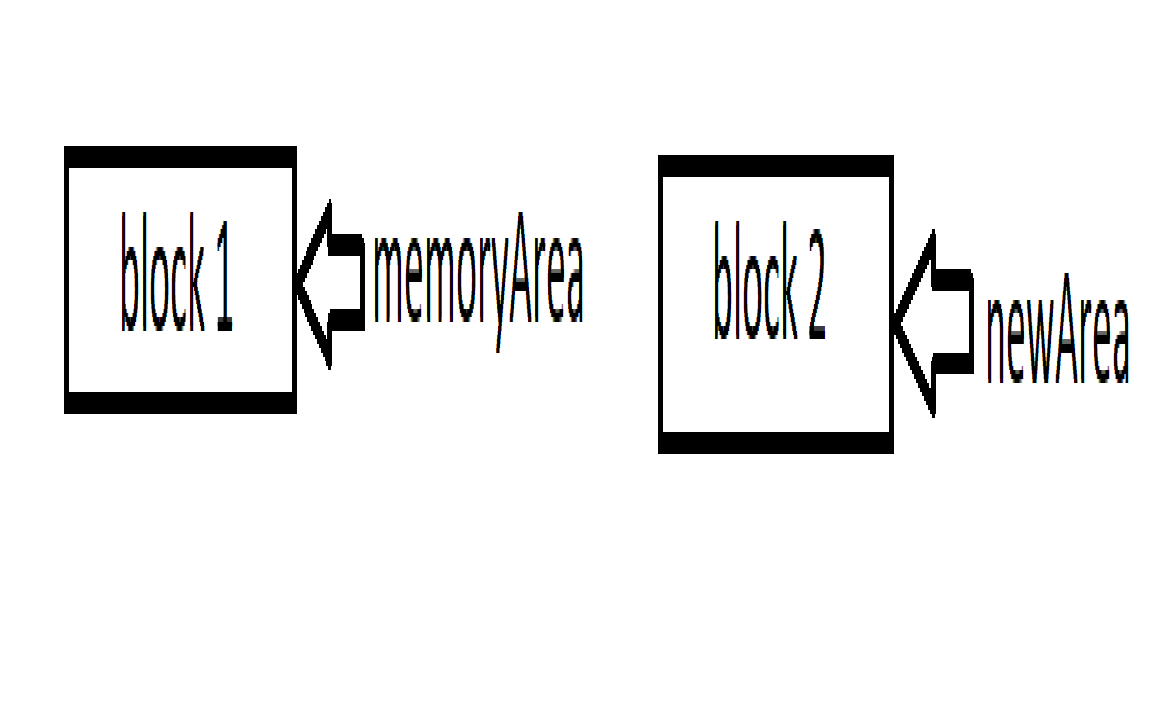
\includegraphics[height=1.2cm,width=6cm]{reassignment1.png}
			\caption{Reassignment error example. Part 1.}
		\end{figure}

		\begin{lstlisting}[language=C++, caption={Reassignment error example. Part 2.}]
		memoryArea = newArea;
		free(memoryArea);
		free(newArea);
		\end{lstlisting}

		\begin{figure}
			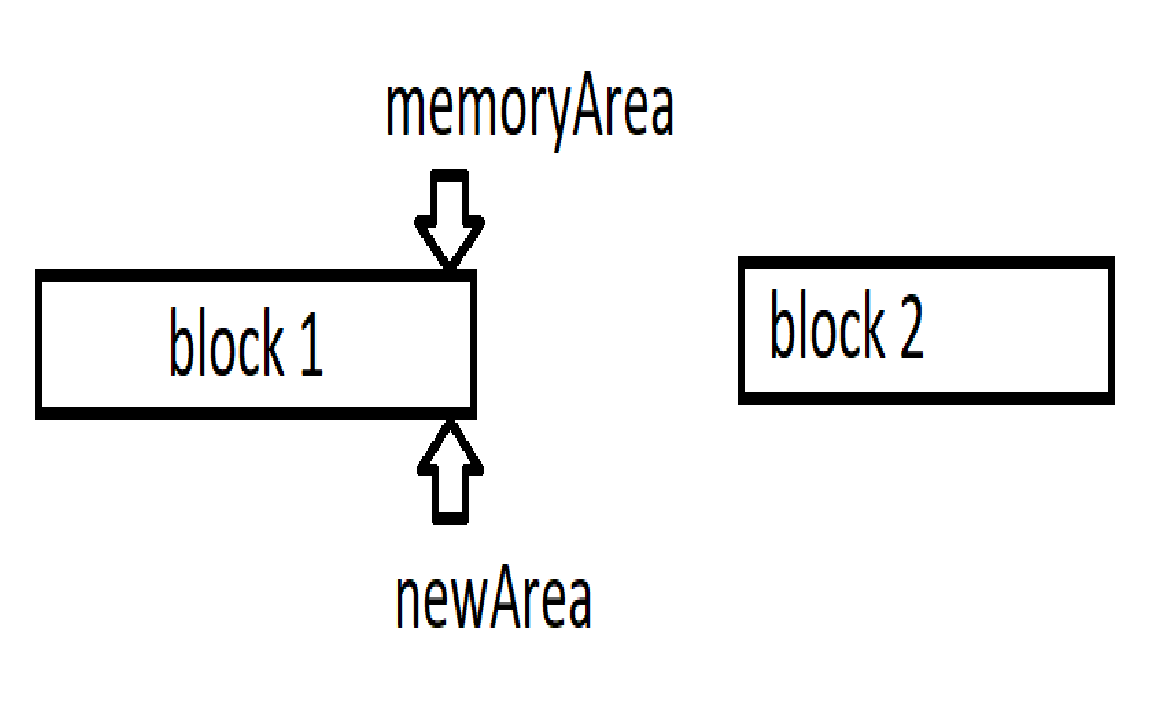
\includegraphics[height=1.5cm,width=5cm]{reassignment2.png}
			\caption{Reassignment error example. Part 2.}
		\end{figure}
	\end{center}
\end{frame}

\begin{frame}[fragile]
	\frametitle{Reassignment. Valgrind output}
	\begin{center}
		\begin{figure}
			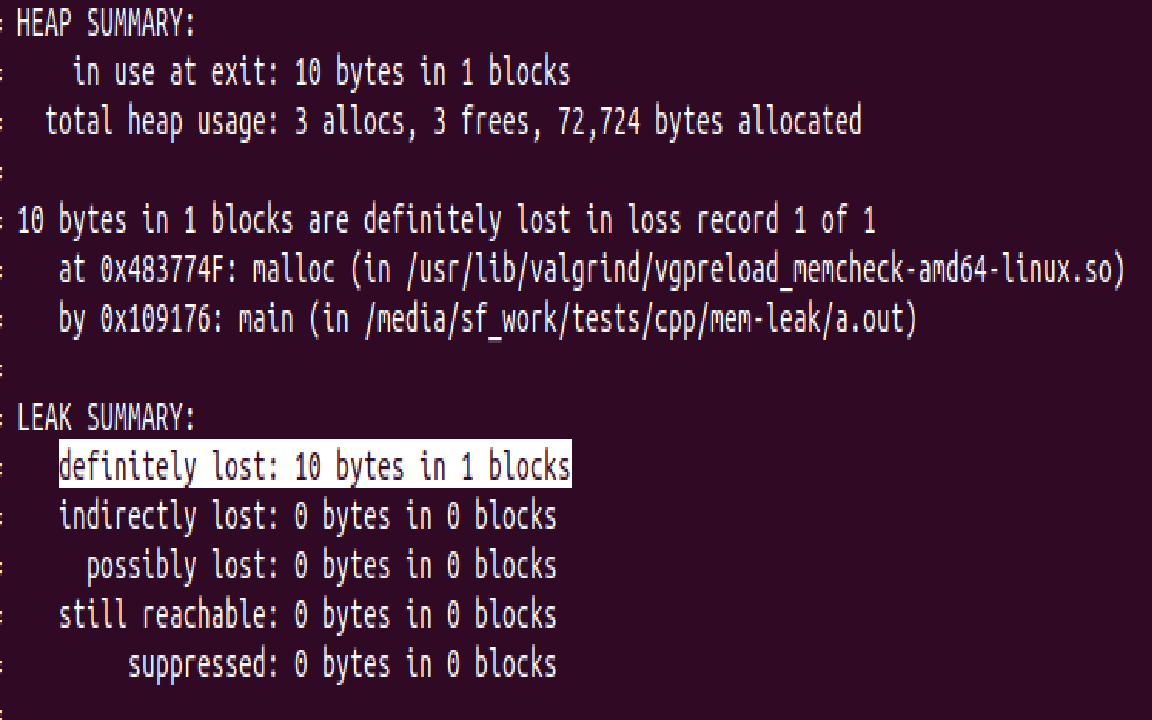
\includegraphics[height=4cm,width=10cm]{reassignment-valgrind.png}
		\end{figure}
	\end{center}
\end{frame}

\subsection{Freeing the parent block first}
\frame{\frametitle{Common mistakes. Freeing the parent block first. The code} 
\begin{itemize}
	\item Reassignment;
	\item \emph{ Freeing the parent block first};
	\item Improper handling of return values;
	\item Many C library functions malloc's memory which MUST be freed;
	\item Forget free or delete after malloc or new operation accordingly;
	\item Inheritance, polymorphism and the wrong delete;
	\item Default copy constructor may not give correct results;
	\item For new[] uses delete (not delete[]).
	\item Out of bounds array;
	\item Forget free static/global variables or resource.
\end{itemize}
}

\begin{frame}[fragile]
\frametitle{Freeing the parent block first. The code} 
	\begin{center}
		\begin{lstlisting}[language=C++]
		char **memoryArea = (char **)malloc(10);
		char *newArea =  (char *)malloc(10);
		memoryArea[2] = newArea;

		free(memoryArea);
		\end{lstlisting}

		\begin{figure}
			\caption{Parent block and child block}
			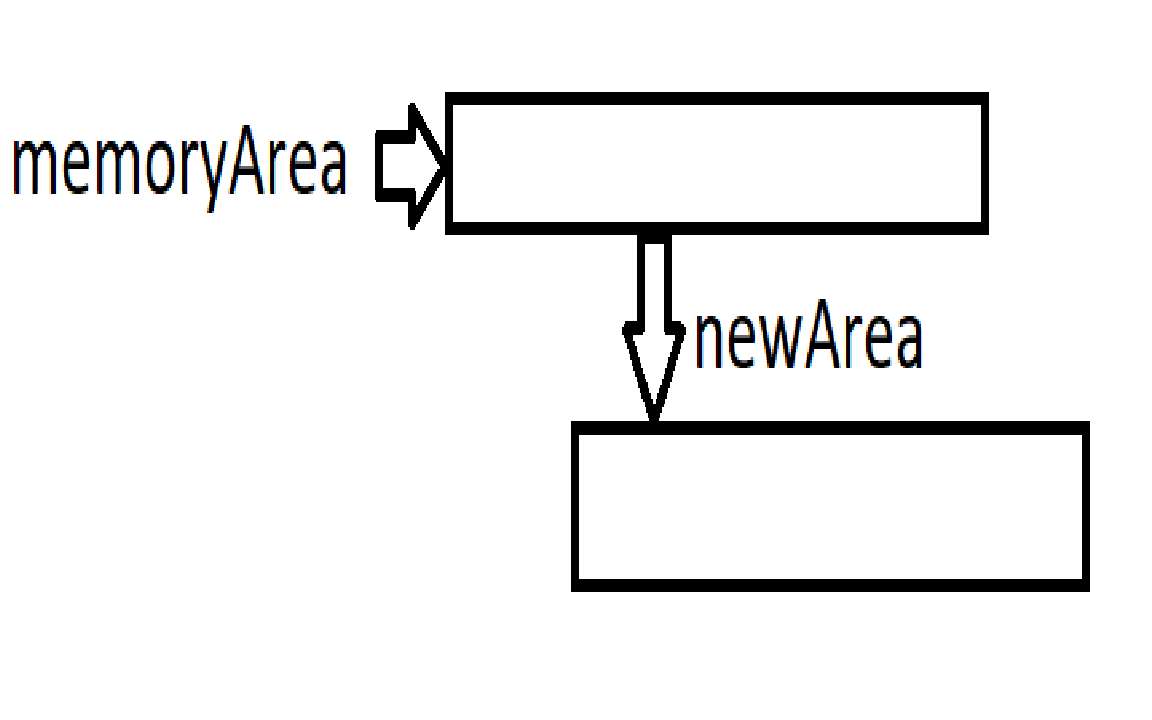
\includegraphics[height=1cm,width=5cm]{freeing-parent-block-first.png}
		\end{figure}

		\begin{figure}
			\caption{Parent block freed}
			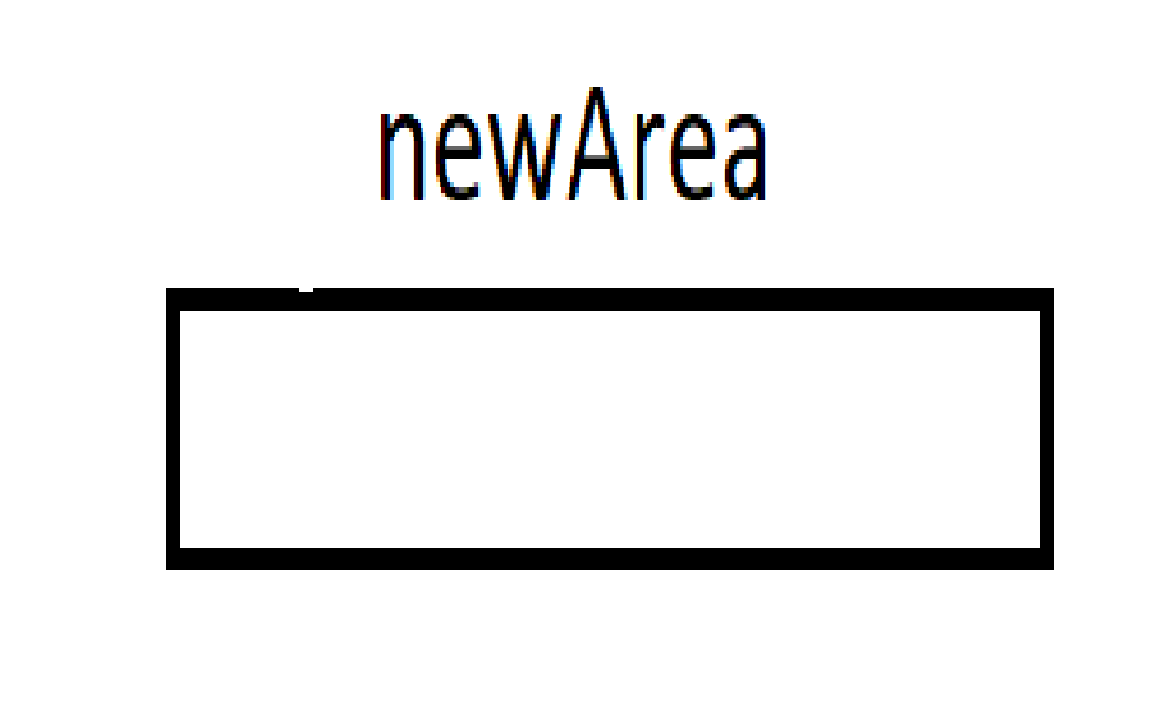
\includegraphics[height=1cm,width=5cm]{freeing-parent-block-first2.png}
		\end{figure}
	\end{center}
\end{frame}

\begin{frame}[fragile]
	\frametitle{Freeing the parent block first. Valgrind output}
	\begin{center}
		\begin{figure}
			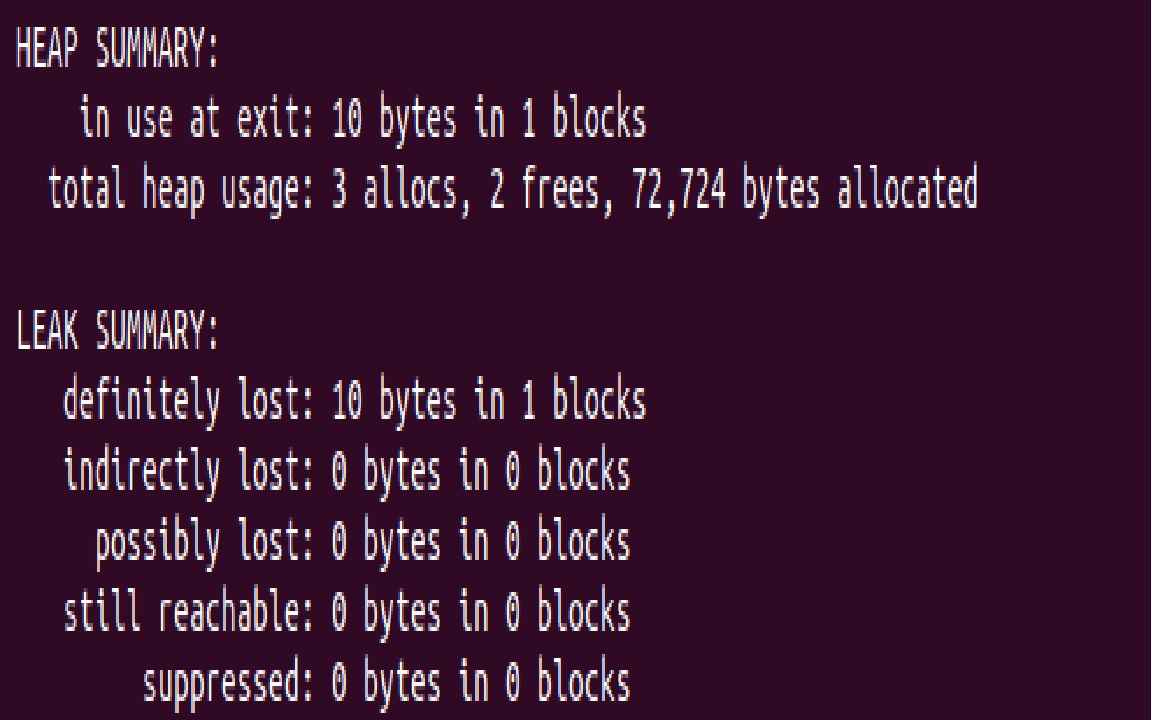
\includegraphics[height=4cm,width=10cm]{freeing-parent-block-first-valgrind.png}
		\end{figure}
	\end{center}
\end{frame}

\subsection{Improper handling of return values}
\frame{\frametitle{Common mistakes. Improper handling of return values} 
\begin{itemize}
	\item Reassignment;
	\item Freeing the parent block first;
	\item \emph{ Improper handling of return values};
	\item Many C library functions malloc's memory which MUST be freed;
	\item Forget free or delete after malloc or new operation accordingly;
	\item Inheritance, polymorphism and the wrong delete;
	\item Default copy constructor may not give correct results;
	\item For new[] uses delete (not delete[]).
	\item Out of bounds array;
	\item Forget free static/global variables or resource.
\end{itemize}
}

\begin{frame}[fragile]
\frametitle{Improper handling of return values. The code} 
	\begin{center}
		\begin{lstlisting}[language=C++]
		char* f()
		{
			char *tmp = static_cast<char *>(malloc(20));
			return tmp;
		}

		int main()
		{
			f();
			return 0;
		}
		\end{lstlisting}
	\end{center}
\end{frame}
% TODO: make description for all valgrind outputs
\begin{frame}[fragile]
	\frametitle{Improper handling of return values. Valgrind output}
	\begin{center}
		\begin{figure}
			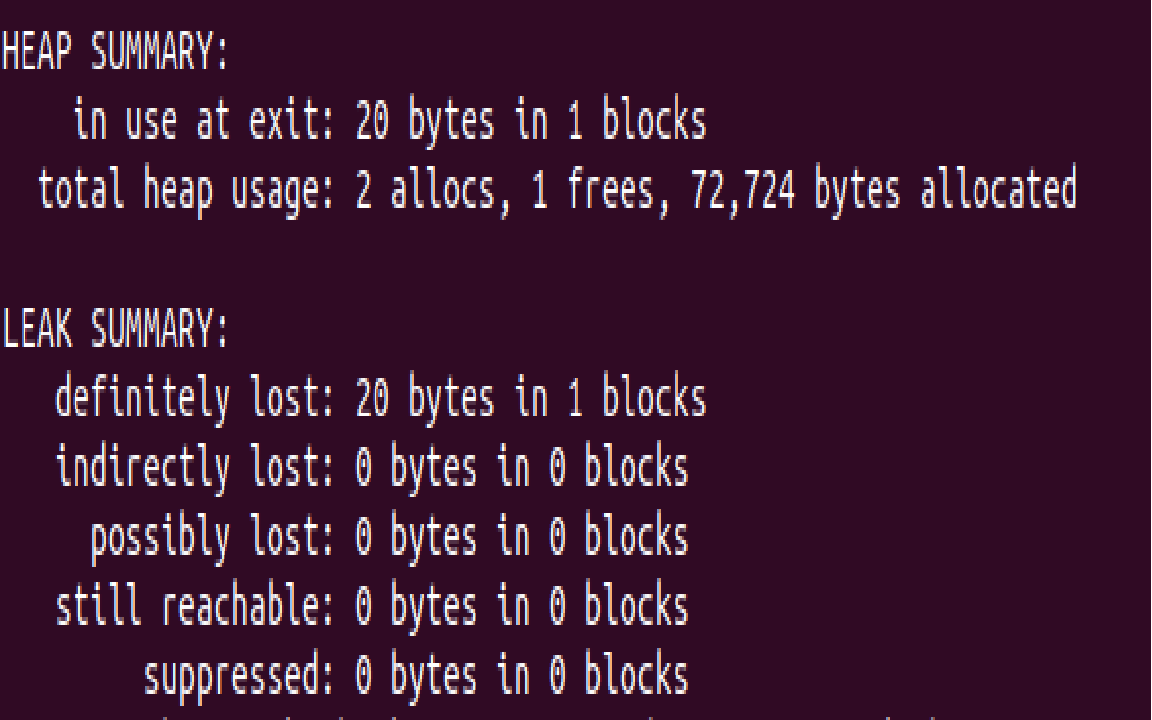
\includegraphics[height=4cm,width=10cm]{improper_handling_of_return_values.png}
		\end{figure}
	\end{center}
\end{frame}

\subsection{Many C library functions malloc's memory which MUST be freed}
\frame{\frametitle{Common mistakes. Many C library functions malloc's memory which MUST be freed}
\begin{itemize}
	\item Reassignment;
	\item Freeing the parent block first;
	\item Improper handling of return values;
	\item \emph{ Many C library functions malloc's memory which MUST be freed};
	\item Forget free or delete after malloc or new operation accordingly;
	\item Inheritance, polymorphism and the wrong delete;
	\item Default copy constructor may not give correct results;
	\item For new[] uses delete (not delete[]);
	\item Out of bounds array;
	\item Forget free static/global variables or resource.
\end{itemize}
}

\begin{frame}[fragile]
\frametitle{Many C library functions malloc's memory which MUST be freed. The code} 
	\begin{center}
		\begin{lstlisting}[language=C++]
			char str[20] = "this is test";
			char *p = strdup(str);
		\end{lstlisting}
	\end{center}
\end{frame}

\begin{frame}[fragile]
	\frametitle{Many C library functions malloc's memory which MUST be freed. Valgrind output}
	\begin{center}
		\begin{figure}
			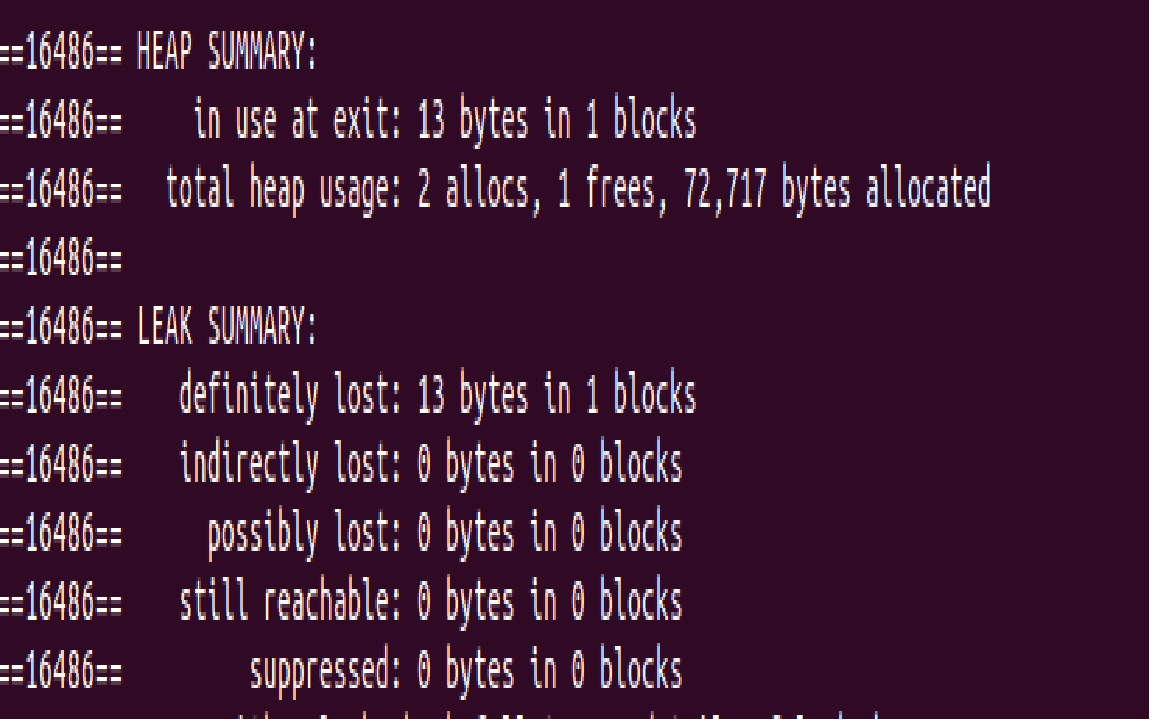
\includegraphics[height=4cm,width=10cm]{c_funcs_which_allocs_mem.png}
		\end{figure}
	\end{center}
\end{frame}

\subsection{Forget free or delete after malloc or new operation accordingly}

\frame{\frametitle{Common mistakes. Forget free or delete after malloc or new operation accordingly}
\begin{itemize}
	\item Reassignment;
	\item Freeing the parent block first;
	\item Improper handling of return values;
	\item Many C library functions malloc's memory which MUST be freed;
	\item \emph{ Forget free or delete after malloc or new operation accordingly};
	\item Inheritance, polymorphism and the wrong delete;
	\item Default copy constructor may not give correct results;
	\item For new[] uses delete (not delete[]);
	\item Out of bounds array;
	\item Forget free static/global variables or resource.
\end{itemize}
}

\begin{frame}[fragile]
\frametitle{Forget free or delete after malloc or new operation accordingly. The code} 
	\begin{center}
		\begin{lstlisting}[language=C++]
		void f()
		{
			int *ar = new int[15];
		}
		
		int main()
		{
			f();
			return 0;
		}
		\end{lstlisting}
	\end{center}
\end{frame}

\begin{frame}[fragile]
	\frametitle{Forget free or delete after malloc or new operation accordingly. Valgrind output}
	\begin{center}
		\begin{figure}
			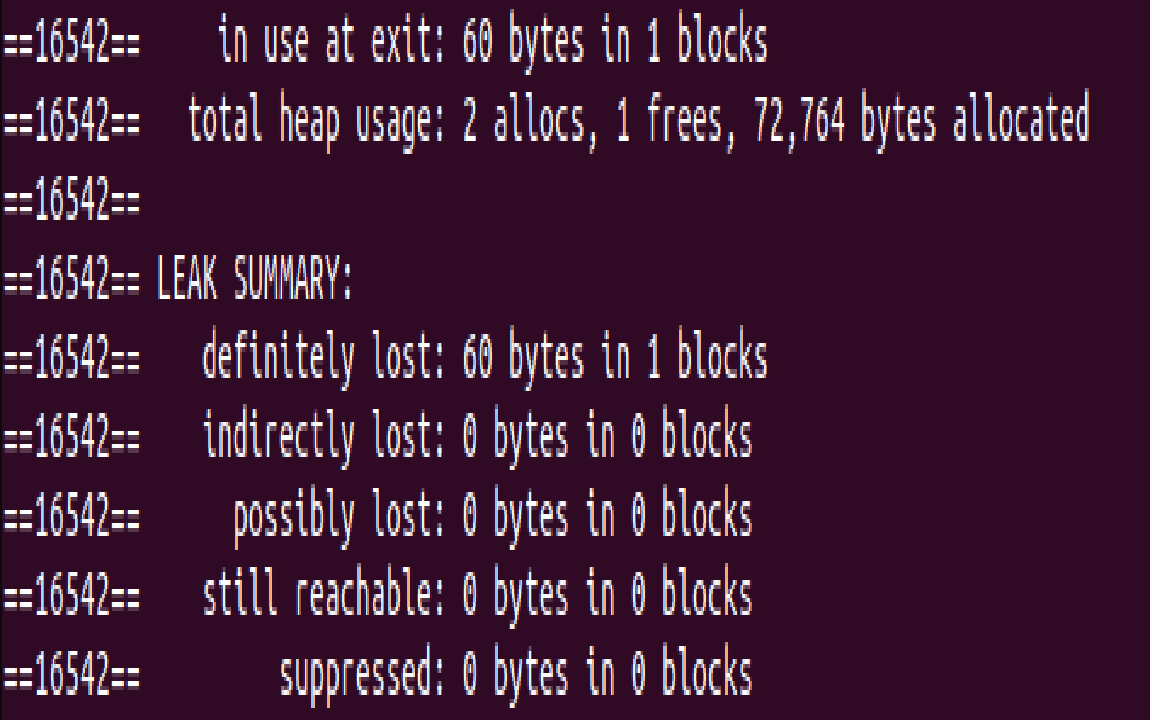
\includegraphics[height=4cm,width=10cm]{forget.png}
		\end{figure}
	\end{center}
\end{frame}

\subsection{Inheritance, polymorphism and the wrong delete}

\frame{\frametitle{Common mistakes. Inheritance, polymorphism and the wrong delete}
\begin{itemize}
	\item Reassignment;
	\item Freeing the parent block first;
	\item Improper handling of return values;
	\item Many C library functions malloc's memory which MUST be freed;
	\item Forget free or delete after malloc or new operation accordingly;
	\item \emph{ Inheritance, polymorphism and the wrong delete};
	\item Default copy constructor may not give correct results;
	\item For new[] uses delete (not delete[]);
	\item Out of bounds array;
	\item Forget free static/global variables or resource.
\end{itemize}
}

\begin{frame}[fragile]
\frametitle{Inheritance, polymorphism and the wrong delete. The code} 
	\begin{center}
		\begin{lstlisting}[language=C++]
class Base
{
};

class Derived: public Base
{
private:
	int *mData;
public:
	Derived() { mData = new int[20]; }
	~Derived() { delete [] mData; }
};

int main()
{
	Derived *d = new Derived();
	Base *b = static_cast<Base *>(d);
	delete b;

	return 0;
}
		\end{lstlisting}
	\end{center}
\end{frame}

% A class that declares or inherits a virtual function is called a polymorphic class. 
\begin{frame}[fragile]
	\frametitle{Inheritance, polymorphism and the wrong delete. Valgrind output}
	\begin{center}
		\begin{figure}
			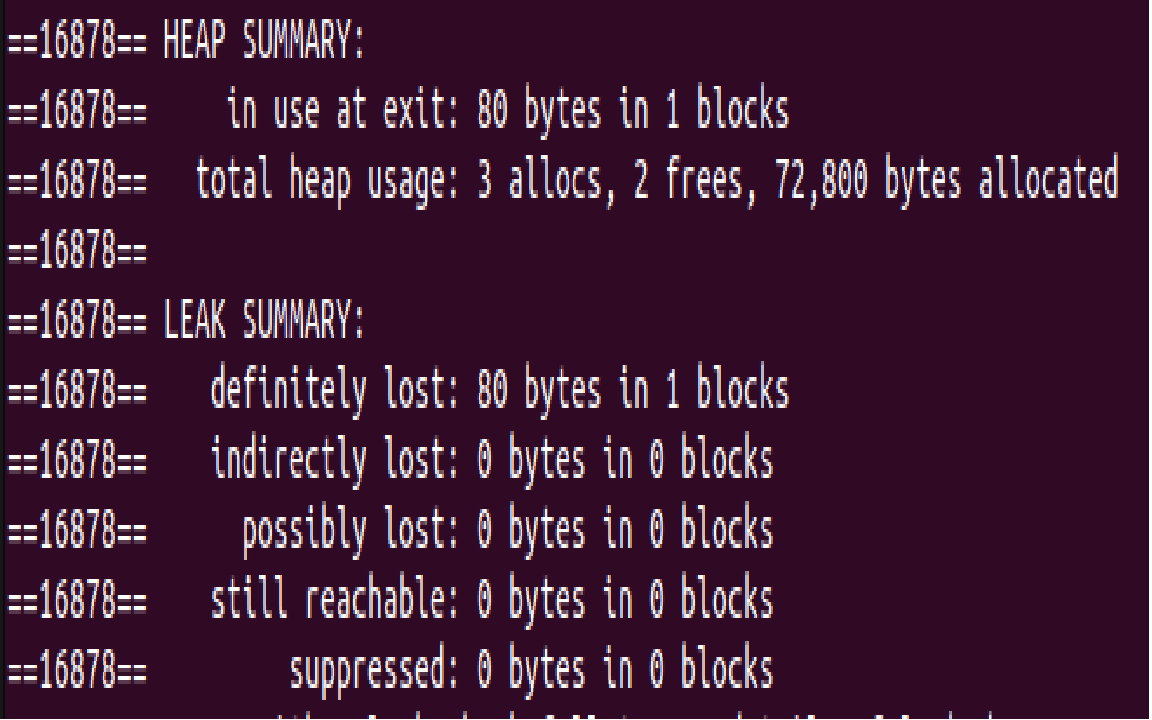
\includegraphics[height=4cm,width=10cm]{virtual_destructor.png}
		\end{figure}
	\end{center}
\end{frame}


\subsection{Default copy constructor may not give correct results}
\frame{\frametitle{Common mistakes. Default copy constructor may not give correct results}
\begin{itemize}
	\item Reassignment;
	\item Freeing the parent block first;
	\item Improper handling of return values;
	\item Many C library functions malloc's memory which MUST be freed;
	\item Forget free or delete after malloc or new operation accordingly;
	\item Inheritance, polymorphism and the wrong delete;
	\item \emph{ Default copy constructor may not give correct results};
	\item For new[] uses delete (not delete[]);
	\item Out of bounds array;
	\item Forget free static/global variables or resource.
\end{itemize}
}

\begin{frame}[fragile]
	\frametitle{Default copy constructor may not give correct results}
	\begin{center}
		\begin{lstlisting}[language=C++]
class A
{
private:
	int *mData;
	int mN;

public:
	A(int N): mN(N) { mData = new int[mN]; }
};

int main()
{
	A a1(5);
	A a2(a1);
	A a3(5);

	a3 = a2;

	return 0;
}
		\end{lstlisting}
	\end{center}
\end{frame}

% A class that declares or inherits a virtual function is called a polymorphic class. 
\begin{frame}[fragile]
	\frametitle{Default copy constructor may not give correct results}
	\begin{center}
		\begin{figure}
			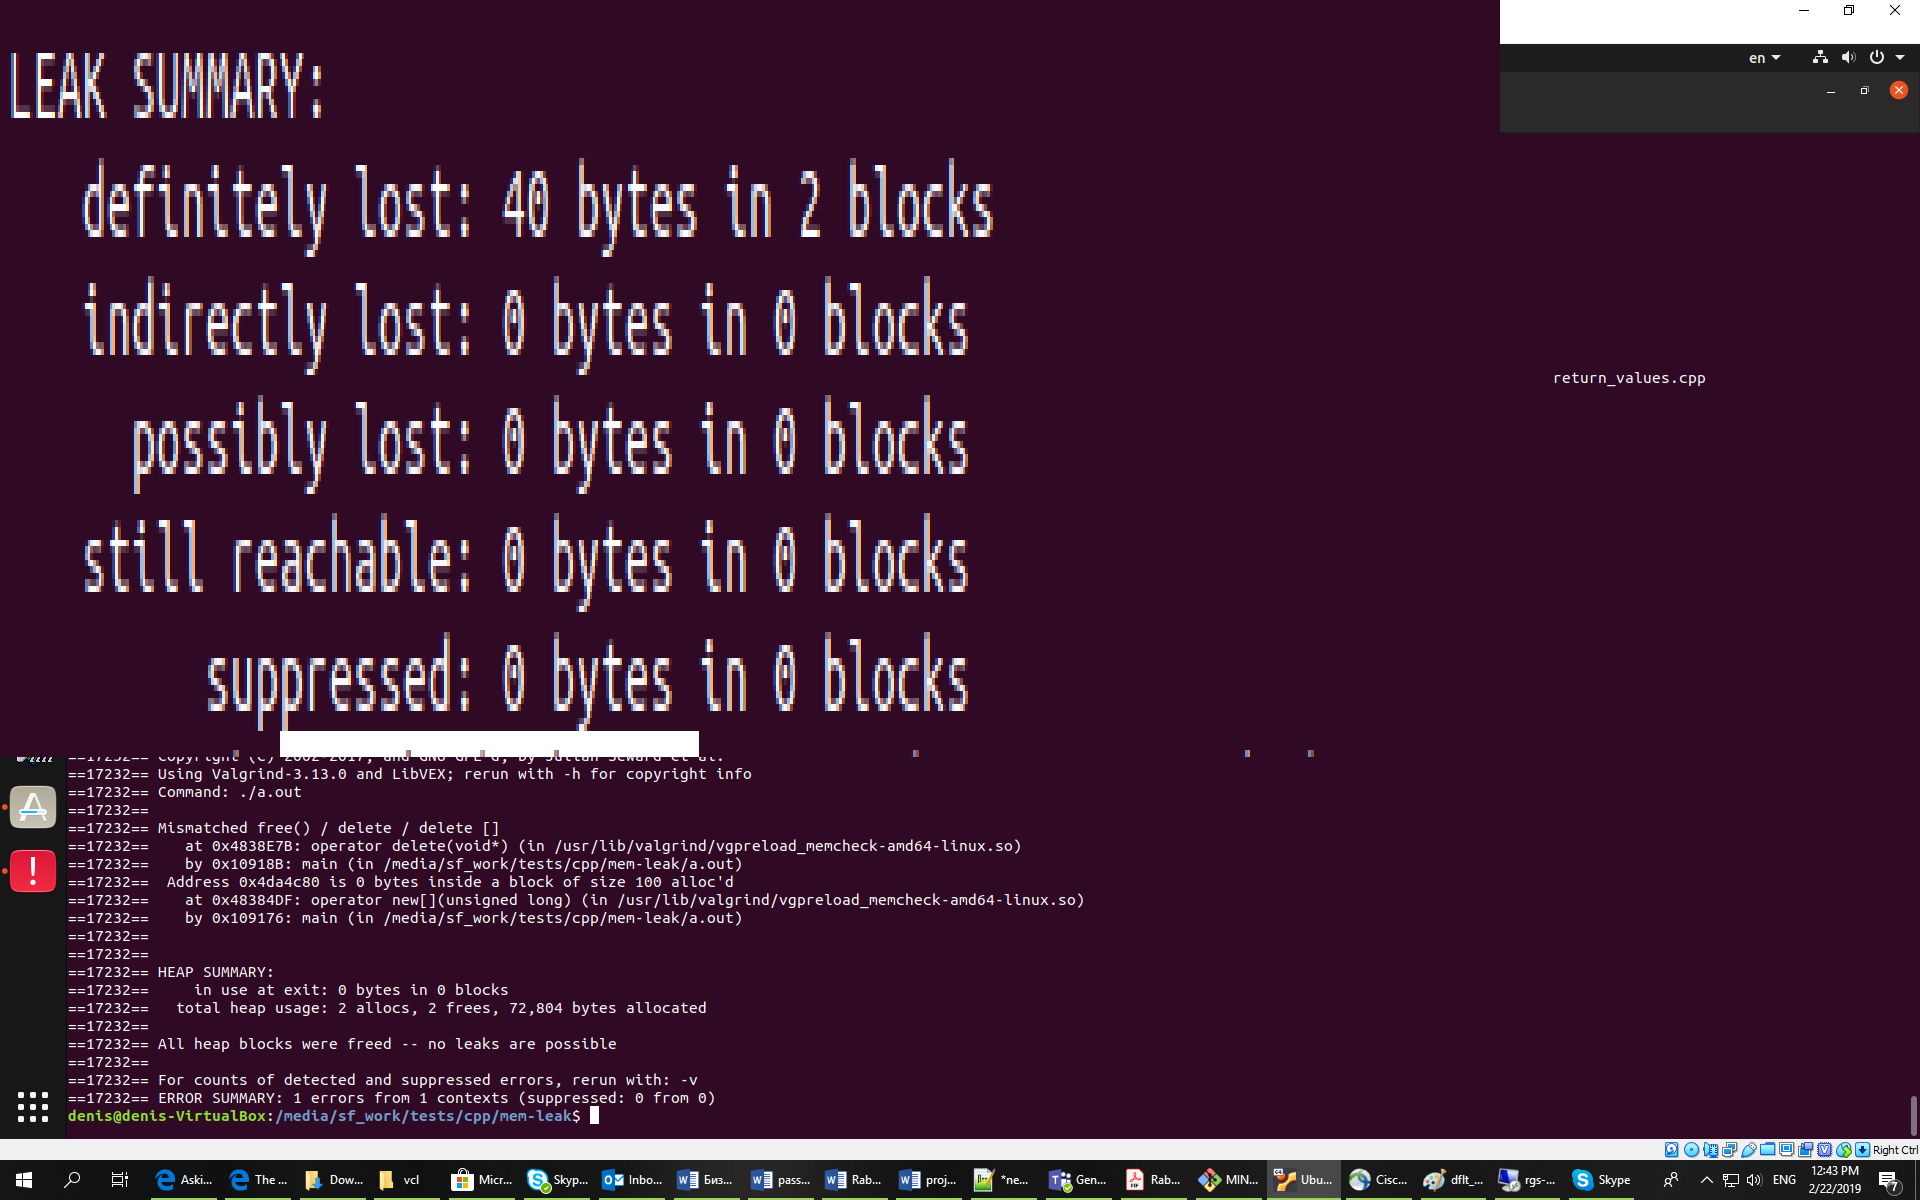
\includegraphics[height=4cm,width=10cm]{dflt_constructor.png}
		\end{figure}
	\end{center}
\end{frame}

\subsection{For new[] uses delete (not delete[]}
\frame{\frametitle{Common mistakes. For new[] uses delete (not delete[])}
\begin{itemize}
	\item Reassignment;
	\item Freeing the parent block first;
	\item Improper handling of return values;
	\item Many C library functions malloc's memory which MUST be freed;
	\item Forget free or delete after malloc or new operation accordingly;
	\item Inheritance, polymorphism and the wrong delete;
	\item Default copy constructor may not give correct results;
	\item \emph{ For new[] uses delete (not delete[])};
	\item Out of bounds array;
	\item Forget free static/global variables or resource.
\end{itemize}
}

\begin{frame}[fragile]
	\frametitle{For new[] uses delete (not delete[])}
	\begin{center}
		\begin{lstlisting}[language=C++]
	char *ar = new char[100];
	delete ar;
		\end{lstlisting}
	\end{center}
\end{frame}

% A class that declares or inherits a virtual function is called a polymorphic class. 
\begin{frame}[fragile]
	\frametitle{For new[] uses delete (not delete[])}
	\begin{center}
		\begin{figure}
			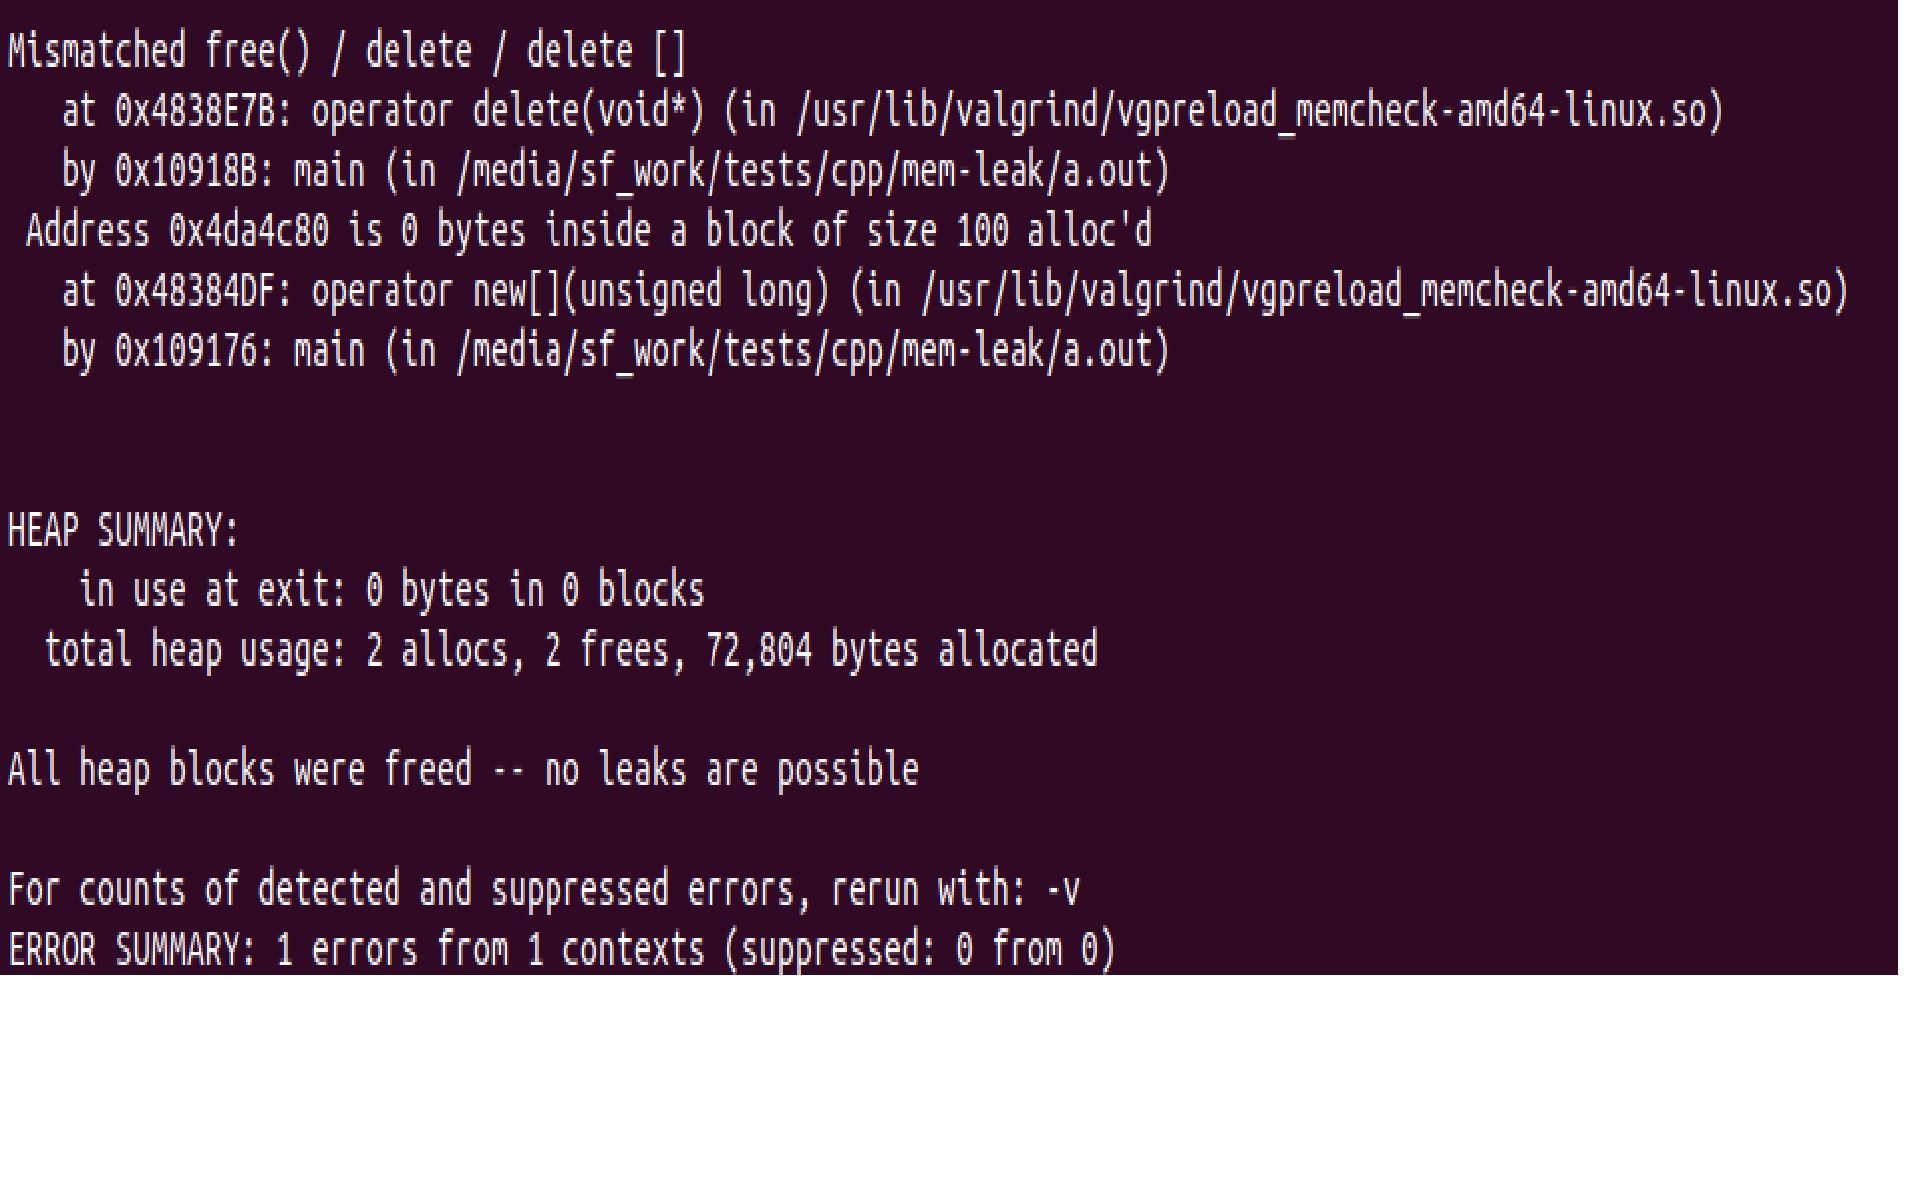
\includegraphics[height=4cm,width=10cm]{delete.png}
		\end{figure}
	\end{center}
\end{frame}

\subsection{Out of bounds array}
\frame{\frametitle{Common mistakes. Out of bounds array}
\begin{itemize}
	\item Reassignment;
	\item Freeing the parent block first;
	\item Improper handling of return values;
	\item Many C library functions malloc's memory which MUST be freed;
	\item Forget free or delete after malloc or new operation accordingly;
	\item Inheritance, polymorphism and the wrong delete;
	\item Default copy constructor may not give correct results;
	\item For new[] uses delete (not delete[]);
	\item \emph{ Out of bounds array};
	\item Forget free static/global variables or resource.
\end{itemize}
}

\begin{frame}[fragile]
	\frametitle{Out of bounds array}
	\begin{center}
		\begin{lstlisting}[language=C++]
int f()
{
	return 10;
}

int main()
{
	int a[3];
	a[f()] = 10;
	return 0;
}
		\end{lstlisting}
	\end{center}
	\begin{center}
		\begin{figure}
			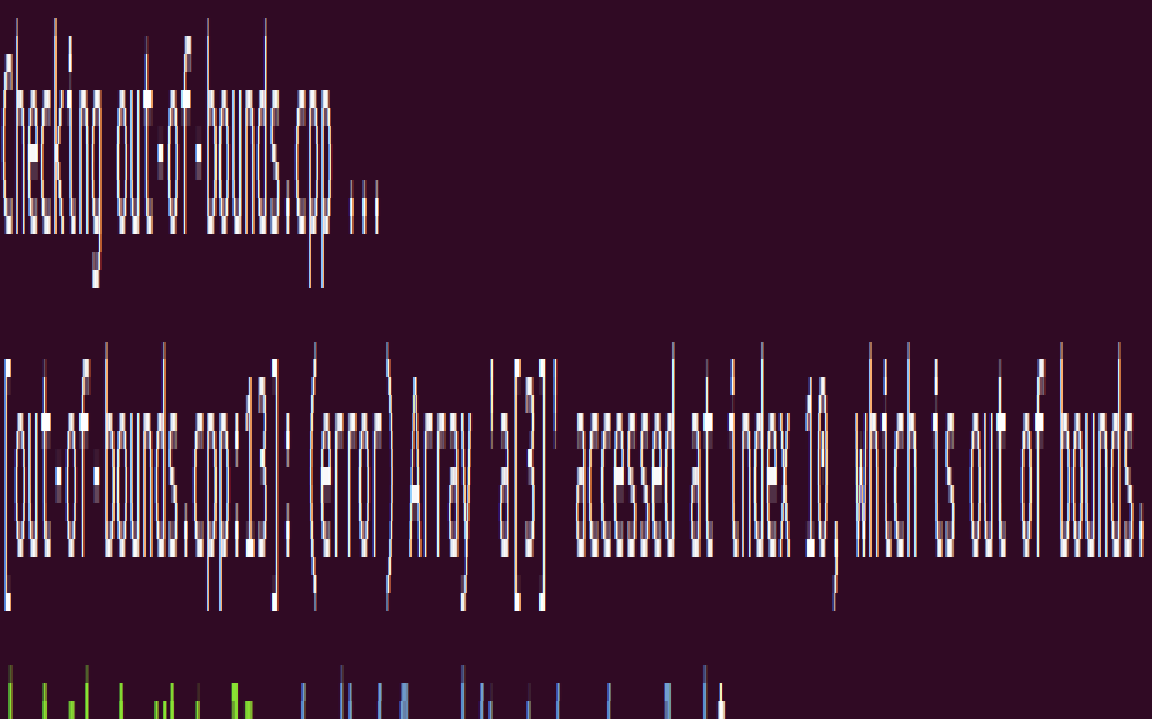
\includegraphics[height=0.7cm,width=10cm]{cppcheck.png}
		\end{figure}
	\end{center}
\end{frame}

\subsection{Forget free static/global variables or resource}
\frame{\frametitle{Common mistakes. Out of bounds array}
\begin{itemize}
	\item Reassignment;
	\item Freeing the parent block first;
	\item Improper handling of return values;
	\item Many C library functions malloc's memory which MUST be freed;
	\item Forget free or delete after malloc or new operation accordingly;
	\item Inheritance, polymorphism and the wrong delete;
	\item Default copy constructor may not give correct results;
	\item For new[] uses delete (not delete[]);
	\item Out of bounds array;
	\item \emph{ Forget free static/global variables or resource}.
\end{itemize}
}

% A class that declares or inherits a virtual function is called a polymorphic class. 
\begin{frame}[fragile]
	\frametitle{Forget free static/global variables or resource}
	\begin{center}
		\begin{lstlisting}[language=C++]
void foo(void)
{
	static char *working_buf = NULL;
	if (!working_buf) {
		working_buf = (char *) malloc(16 * 1024);
	}
}

int main()
{
	foo();
	return 0;
}

		\end{lstlisting}
	\end{center}

	\begin{center}
		\begin{figure}
			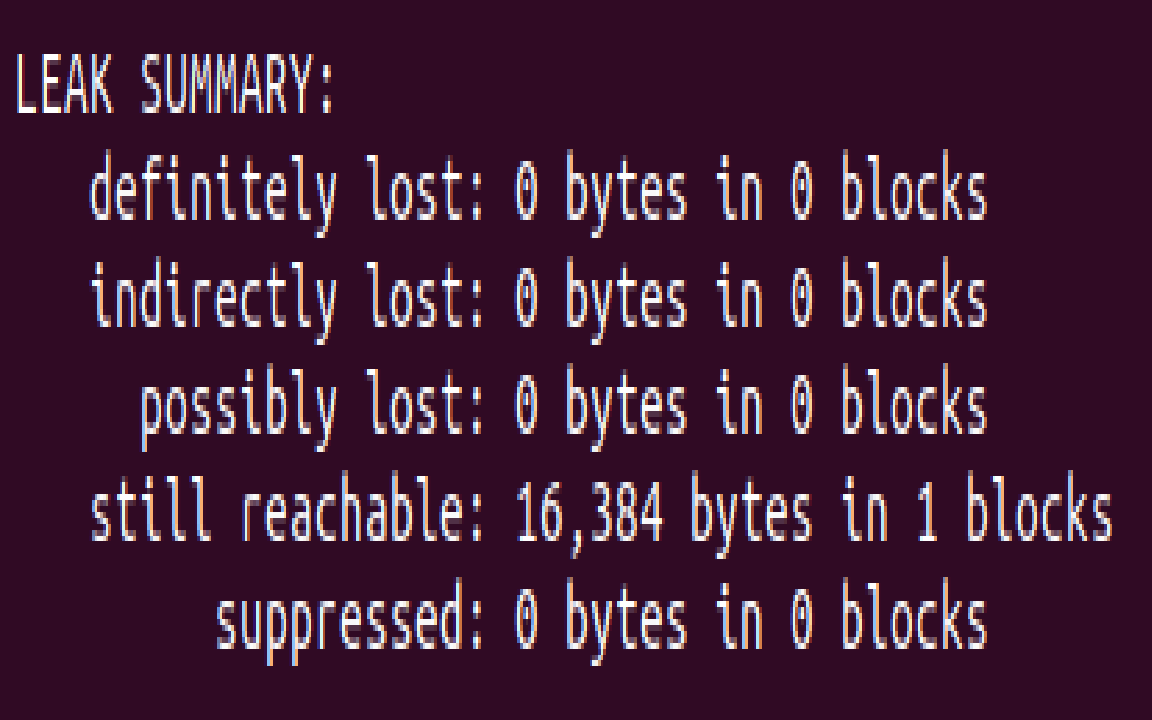
\includegraphics[height=1.5cm,width=11cm]{forget_free_static.png}
		\end{figure}
	\end{center}
\end{frame}

% TODO: wrong example. Must be file opening
\begin{frame}[fragile]
	\frametitle{Forget free static/global variables or resource}
	\begin{center}
		\begin{lstlisting}[language=C++]
void foo(void)
{
	return 1;
}

int main()
{
	foo();
	return 0;
}

		\end{lstlisting}
	\end{center}

	\begin{center}
		\begin{figure}
			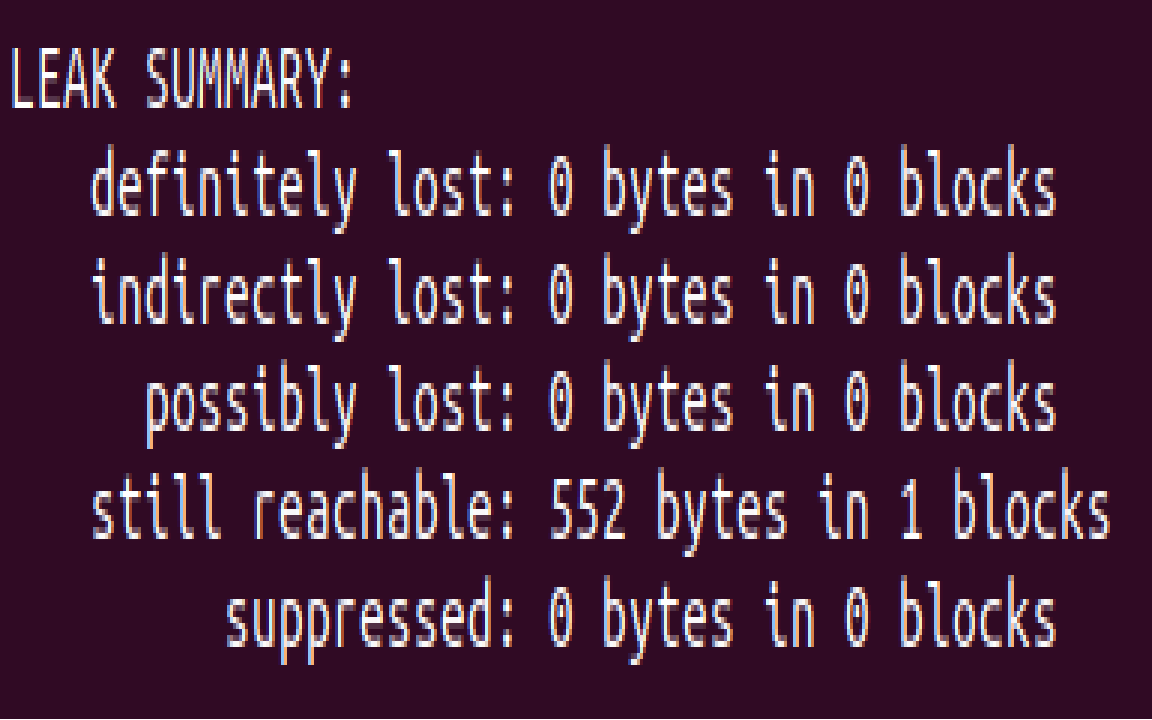
\includegraphics[height=1.5cm,width=11cm]{forget_free_static2.png}
		\end{figure}
	\end{center}
\end{frame}

\section{Tips to avoid problems}
\begin{frame}[fragile]
	\frametitle{}
	\begin{center}
		\begin{exampleblock}{}
			Use smart pointers (shared\_ptr for example).
		\end{exampleblock}
		\begin{exampleblock}{}
			Write own copy constructor for deep copy.
		\end{exampleblock}
		\begin{exampleblock}{}
			RAII idiom (resource aquision is initialisation).
		\begin{lstlisting}[language=C++]
		class RaiiDbExample
		{
		private:
			DataBase mDb;
		public:
			RaiiDbExample() {mDb.connect();}
			~RaiiDbExample() {mDb.disconnect();}
		}

		\end{lstlisting}
	\end{center}
		\end{exampleblock}
		\begin{exampleblock}{}
			Use virtual destructors.
		\end{exampleblock}
		\begin{exampleblock}{}
		Right using of delete[] operator
		\end{exampleblock}
	\end{center}
\end{frame}

\end{document}

